% Created 2017-09-20 Wed 13:20
% Intended LaTeX compiler: pdflatex
\documentclass[presentation]{beamer}
\usepackage{amsmath}
\usepackage{tikz}
\usepackage{hyperref}
\usetheme[height=20pt]{Rochester}
\date{\today}
\title{Search}
\author{A.I. Society at UTDallas}
\begin{document}
\begin{frame}
  \maketitle
\end{frame}
\begin{frame}{Outline}
  \tableofcontents
\end{frame}
\section{Setup}
\begin{frame}
  \frametitle{Setup}
    
\end{frame}
\section{Introduction}
\begin{frame}
  \frametitle{Introduction}
  What does it mean to search?\\
  \begin{figure}
    \centering
    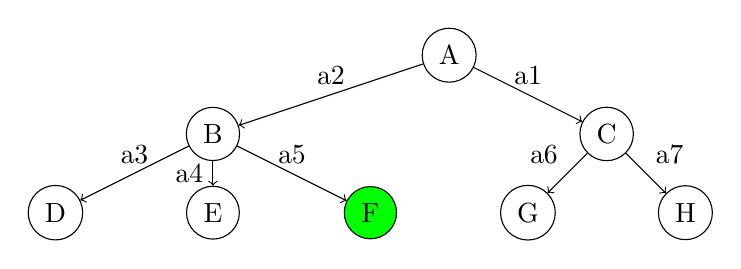
\begin{tikzpicture}
      \node[shape=circle,draw=black](A) at (0,0) {A};
      \node[shape=circle,draw=black](B) at (-3, -1) {B};
      \node[shape=circle,draw=black](C) at (2, -1) {C};
      \node[shape=circle,draw=black](D) at (-5,-2) {D};
      \node[shape=circle,draw=black](E) at (-3, -2) {E};
      \node[shape=circle,draw=black,fill=green](F) at (-1, -2) {F};
      \node[shape=circle,draw=black](G) at (1,-2) {G};
      \node[shape=circle,draw=black](H) at (3, -2) {H};

      \path [->] (A) edge node[above] {a1} (C);
      \path [->] (A) edge node[above] {a2} (B);
      \path [->] (B) edge node[above] {a3} (D);
      \path [->] (B) edge node[left] {a4} (E);
      \path [->] (B) edge node[above] {a5} (F);
      \path [->] (C) edge node[above left] {a6} (G);
      \path [->] (C) edge node[above right] {a7} (H);
    \end{tikzpicture}
  \end{figure}
\end{frame}

\begin{frame}{Problems}
  \begin{itemize}
  \item What Problems can be solved by searching?
    \begin{itemize}
    \item <1-> Chess
    \item <2-> Solving Mazes
    \item <3-> Computer Algebra System
    \end{itemize}
  \item What Problems should we NOT use search?
    \begin{itemize}
    \item <4-> Travelling salesman problem
    \item <5-> Go
    \item <6-> 
    \end{itemize}
  \end{itemize}
\end{frame}
\begin{frame}{Problems}
  
\end{frame}
\section{Breadth First and Depth First Search}
\begin{frame}{Breadth First}
\end{frame}
\begin{frame}
  \frametitle{Depth First}
  
\end{frame}
\begin{frame}{Example Time!}
  TODO: live coding of maze solver
\end{frame}
\begin{frame}
  \frametitle{What's the Difference?}
  
\end{frame}
\section{Bidirectional Search}
\begin{frame}{Bidirectional Search}
  \begin{itemize}
  \item reduce nodes evaluated
  \item only works with a unique goal state
  \end{itemize}
\end{frame}
\section{Heuristics}
\begin{frame}{Heuristics}
  \begin{itemize}
  \item can we make smarter decisions about which nodes to expand?
  \end{itemize}
\end{frame}
\begin{frame}{A*}
\end{frame}
\begin{frame}{Beam Search}
  \begin{itemize}
  \item A* is an extension of breadth first search
  \item Can we improve it by eliminating the limitations that come
    with BFS?
  \end{itemize}
\end{frame}
\begin{frame}{Example Time!}
\end{frame}
\section{Adversarial Search}
\begin{frame}{Adversarial Search}
  \begin{itemize}
  \item A.K.A Minimax
  \item Used to play games
  \item We are not the only one who can choose the next action!
  \end{itemize}
\end{frame}
\begin{frame}{Example Time!}
  text-based Tic Tac Toe example
\end{frame}
\begin{frame}{Alpha Beta Pruning}
  \begin{itemize}
  \item Are there nodes that can can be skipped?
  \item<2-> Yes! Sometimes...
  \end{itemize}
\end{frame}
\begin{frame}
  \frametitle{Chess}
  \begin{itemize}
  \item Add alpha-beta pruning to tic-tac-toe
  \item Transplant algorithm into graphical chess program
  \end{itemize}
\end{frame}
\end{document}
\begin{frame}
  \frametitle{Local Search}
  
\end{frame}
%%% Local Variables:
%%% mode: latex
%%% TeX-master: t
%%% End:
